\Chapter{Rácsok használata a számítógépes játékokban}

% TODO: Definiálni kellene, hogy mi pontosan itt a rács!

\section{Rácsok összehasonlítása}
%\cite{KoordinataRendszer}
%\cite{redblobgamesHexagonalGrids}
%\cite{HexMap}

Legyen szó társasjátékról vagy számítógépes játékról, az egyik leggyakrabban használt rács a négyzetrács. Egyszerű, könnyen kezelhető és jól illeszthető a számítógép kijelzőjére.

A cellák pozícióit sík esetén a \textit{Descartes-féle derékszögű koordináta-rendszer} $(x, y)$ koordináták segítségével határozhatjuk meg.
Kirajzolásához ismernünk kell a cella méreteit (szélesség, magasság) illetve a rács méreteit (oszlopok, sorok száma). 
A nyilvántartáshoz ismernünk kell a viszonyítási pontot (origó), illetve tudnunk kell az objektum pozícióját ($x, y$).

Könnyen kezelhetősége mellett viszont van egy nagy hátránya. Egy négyzetnek nyolc szomszédja van. Oldalain keresztül vízszintesen, valamint függőlegesen 2-2 szomszédja érhető el. További négy szomszédja átlósan található meg. A probléma akkor jelentkezik, amikor megvizsgáljuk a távolságot a különböző szomszédok között. A vizsgálathoz tegyük fel, hogy az oldalak hossza $1$. Ha a négyzetek középpontjához viszonyítunk, akkor a függőlegesen és a vízszintesen lévő szomszédok távolsága $1$, míg az átlósan lévők távolsága $\sqrt{2}$. Ez azért jelent problémát, mert így az átlós szomszédok távolabbra esnek, ezáltal nem lesz arányos a mozgás minden irányban (\ref{fig:SqDistance}. ábra).

\begin{figure}[h!]
\centering
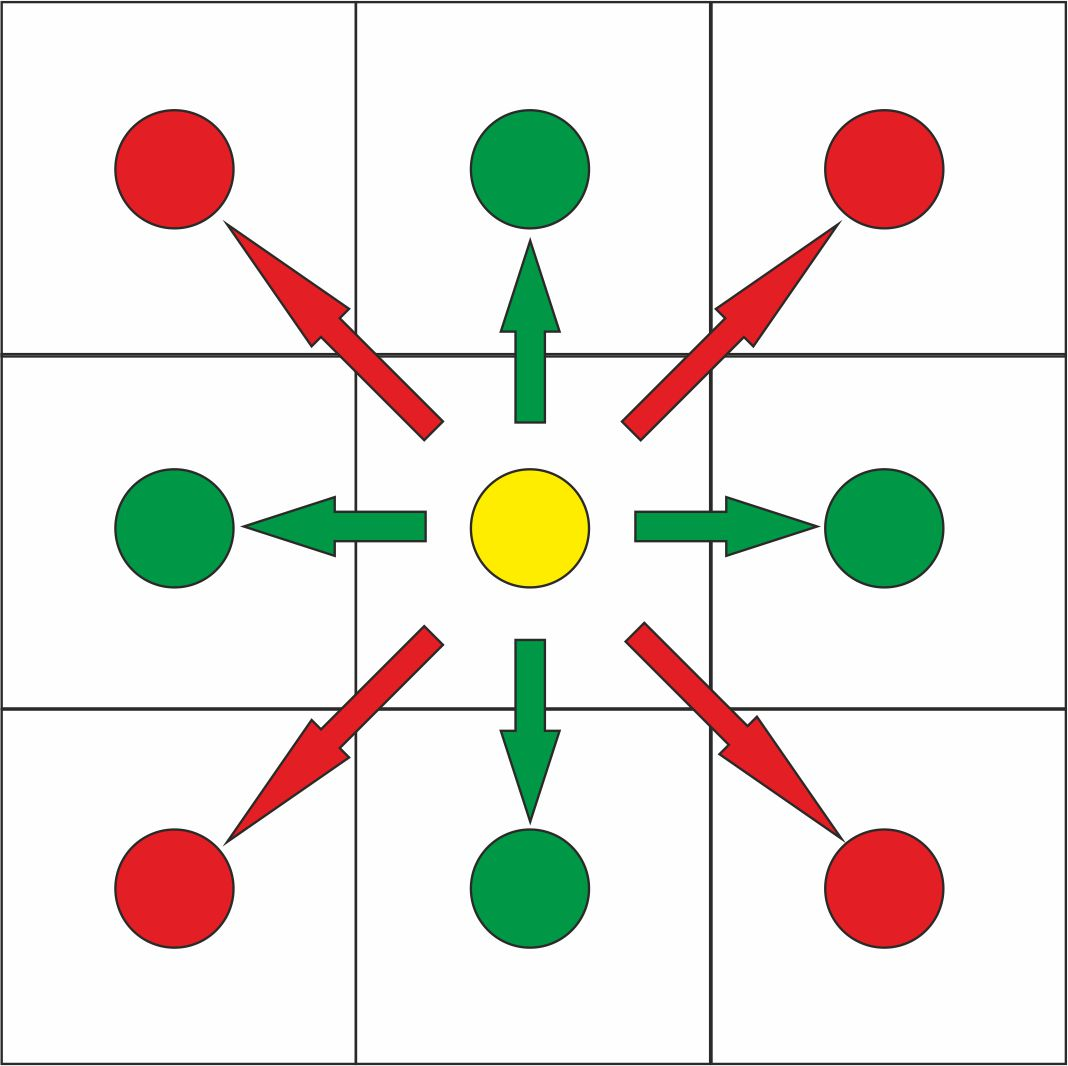
\includegraphics[scale=0.4]{kepek/SqDistance.jpg}
\caption{A szomszédok távolsága a négyzetrács esetén}
\label{fig:SqDistance}
\end{figure}

A két fajta szomszéd közötti különbség miatt vetődnek fel bizonyos kérdések, például, hogy hogyan kezeljük az átlós mozgást? Egyáltalán engedélyezzük-e az átlós mozgást? A mozgás természetessége és arányossága érdekében hogyan érhetnénk el azt, hogy minden szomszéd azonos távolságra legyen egymástól?
\newpage
A problémára több megoldás is létezik, mint például az alábbiak.
\begin{itemize}
\item Nem alkalmazunk átlós mozgást. Ez a legegyszerűbb megoldás, amit az egyszerűsége miatt gyakran használnak.
\item Egy kevésbé elterjedt megoldás, hogy maradunk a négyzeteknél, viszont minden második sort/oszlopot eltolunk az oldal hosszának a felével. Ekkor az összes szomszéd hasonló távolságra kerül (\ref{fig:SqOffsetDistance}. ábra).
\item Amennyiben a játék szabályai és kialakítása lehetővé teszik, számolhatunk $\sqrt{2}$ távolságértékekkel, vagy azok közelítésével is.
\item A leggyakoribb megoldás a hexagonok használata a négyzetek helyett. A négyzethez hasonlítva a hatszögnek csak hat szomszédja van (nyolc helyett). Ezek közül mindegyik oldal szomszéd, és nincs olyan szomszédja ami a sarkokhoz esne. Ezáltal minden szomszéd egyenlően 1 távolságra van.
\end{itemize}

\begin{figure}[h!]
\centering
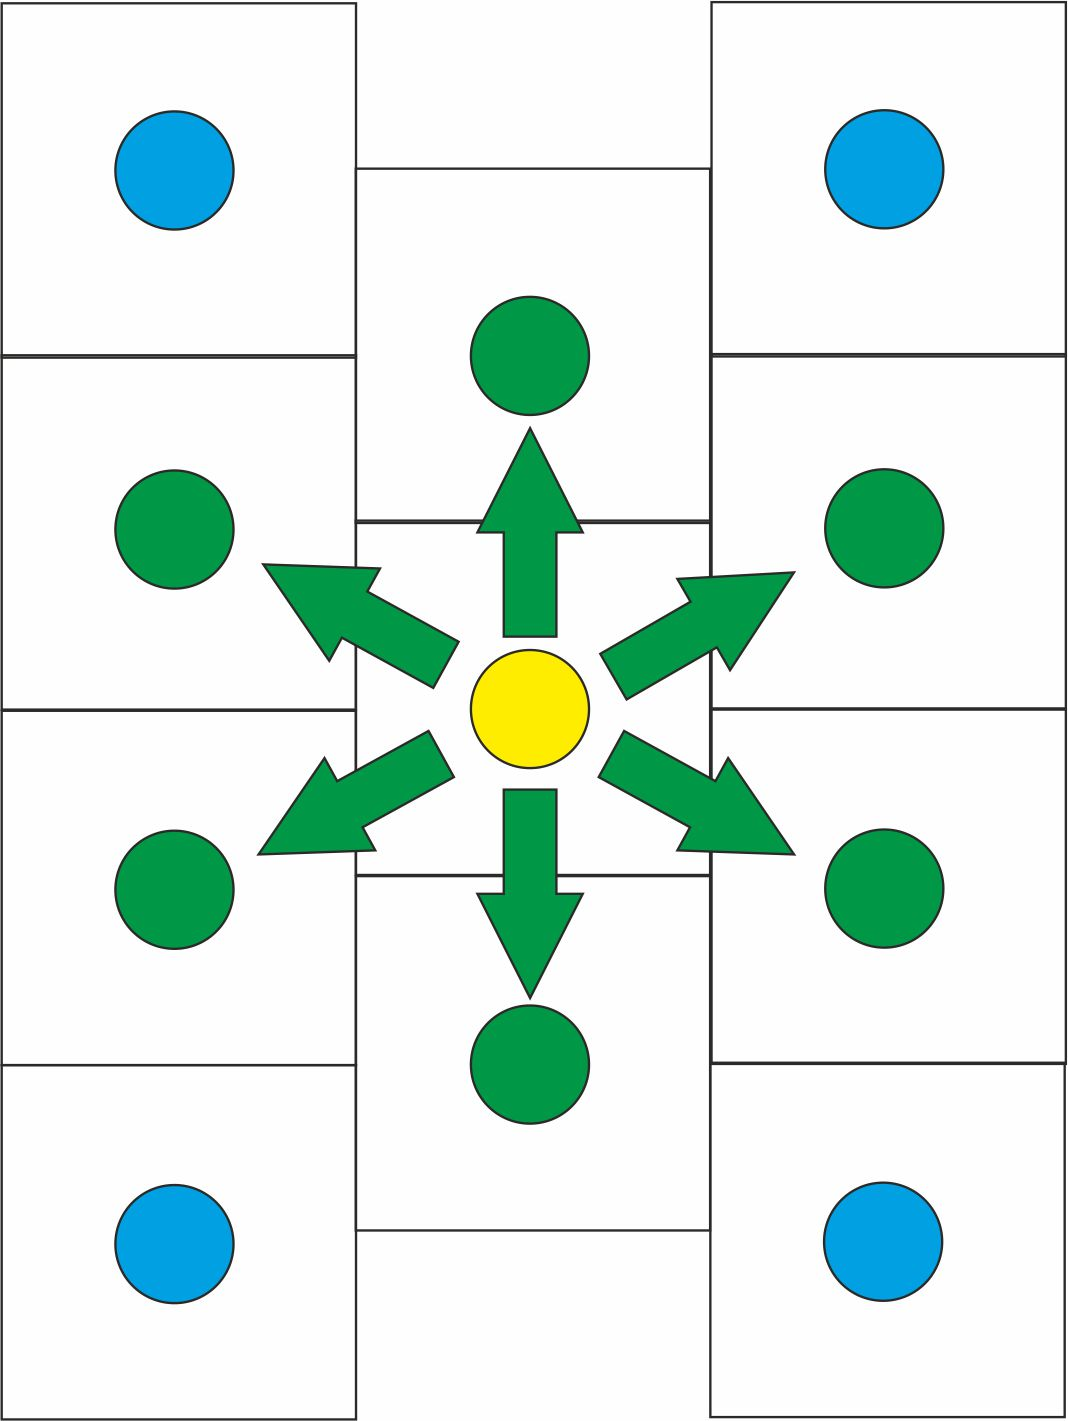
\includegraphics[scale=0.3]{kepek/SqOffsetDistance.jpg}
\caption{Az eltolásos négyzetrács esetén a távolságok}
\label{fig:SqOffsetDistance}
\end{figure}

A hexagonrácsot azért szokták játékokban használni mert kevésbé torzítják a távolságokat mint a négyzetrács. Ez azért van mert nincs átlós szomszédja ellentétben a négyzettel (\ref{fig:HexDistance}. ábra).

\begin{figure}[h!]
\centering
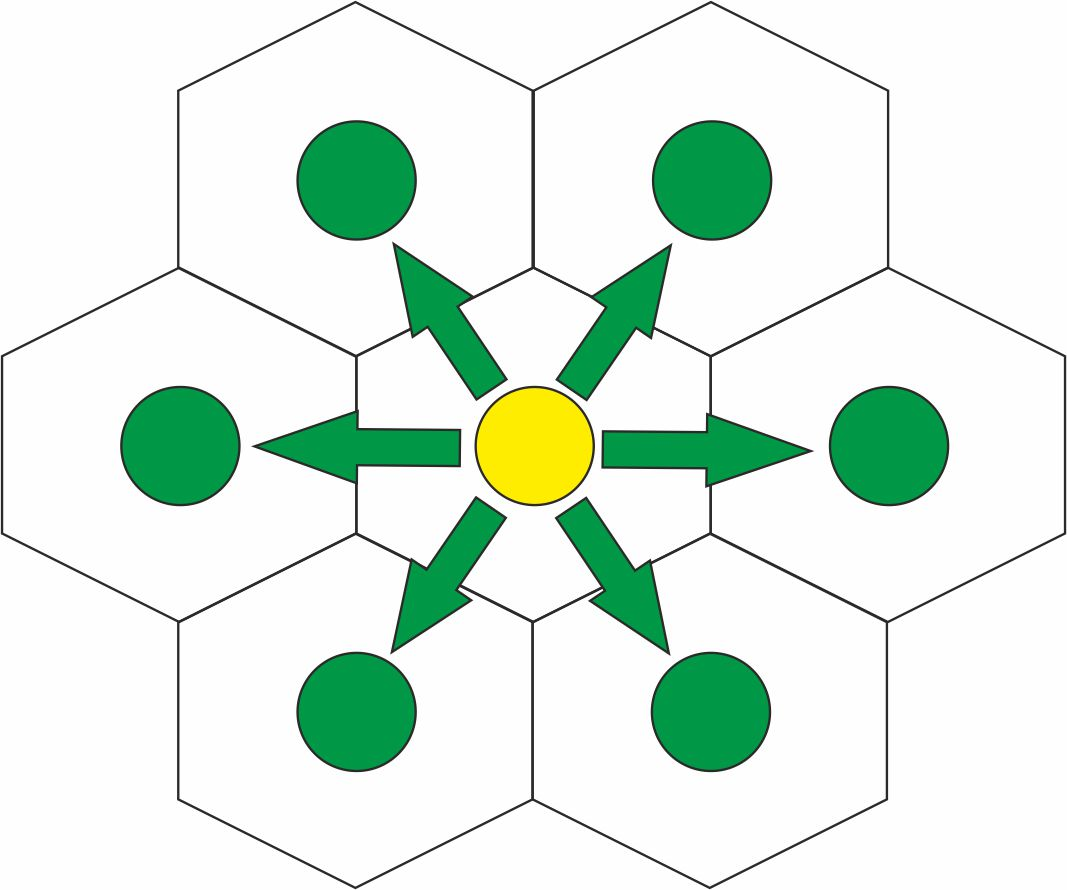
\includegraphics[scale=0.4]{kepek/HexDistance.jpg}
\caption{A szomszédok távolsága a hexagonháló esetén}
\label{fig:HexDistance}
\end{figure}

A fő indok a hexagonháló mellett az eltolt négyzethálóval szemben az, hogy természetesebben adódik a hat lehetséges mozgási iránynak a használata. Sok ember számára zavaró, vagy nem teljesen egyértelmű első ránézésre, hogy hogyan történik a horizontális mozgás az eltolt négyzetrács esetén. Emellett még esztétikailag is kellemesebb érzetet nyújt a felhasználó számára (\ref{fig:SqVsHex}. ábra).
\newpage
\section{Rácsok felhasználása}

Alapvetően mindkét rácsnak megvan a maga helye a játékfejlesztésben.  Mivel a beltéri helyszínek (szobák) és az azon belüli elemek (bútorok) általában téglalap alakúak, praktikusabb a négyzetrács használata. A négyzetrács a falakhoz tökéletesen illeszkedik, ugyanakkor a hexagonok esetében problémák merülnek fel, ugyanis a hexagonok nem fognak szabályosan illeszkedni a falak mentén. Erre kétfajta megoldás létezik: a fal menti hexagonokat elvághatjuk, vagy másik megoldás, ha nem töltjük ki a fennmaradó helyeket.

\begin{figure}[h!]
\centering
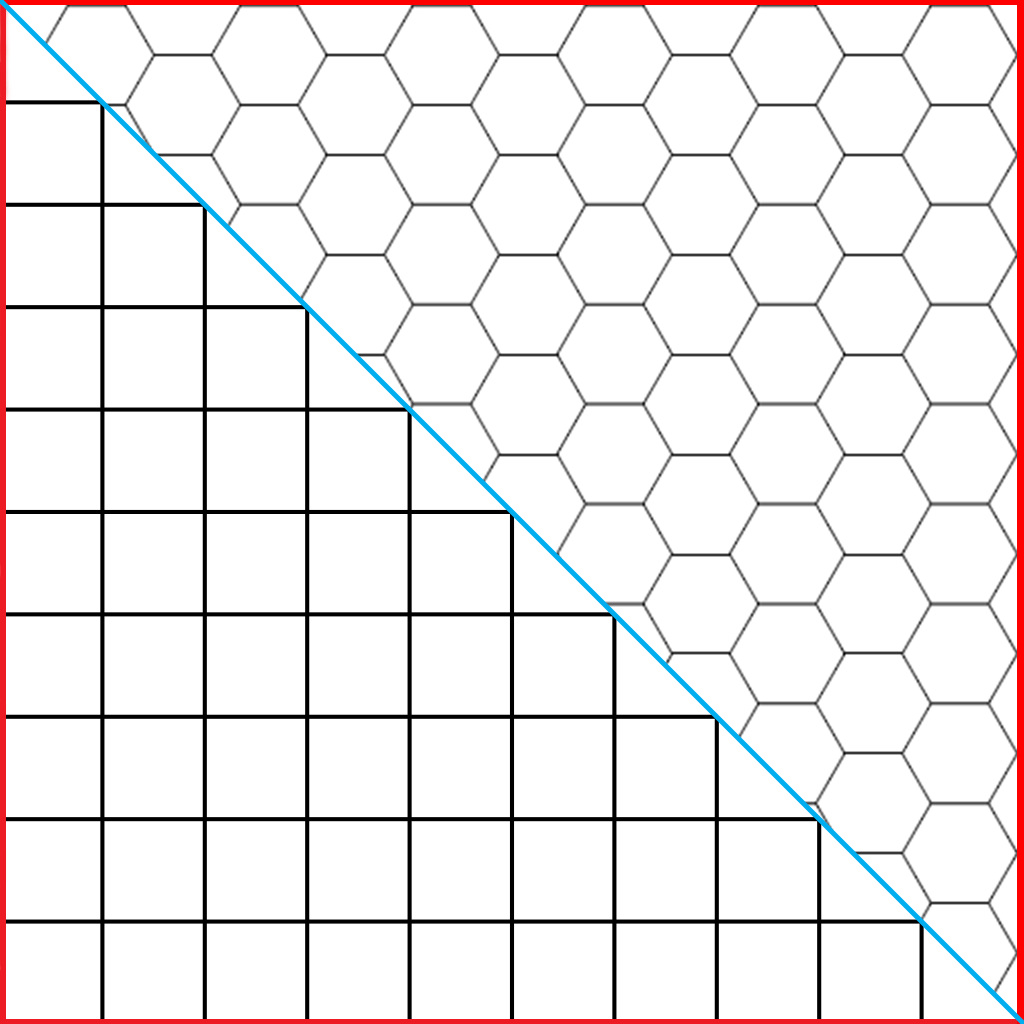
\includegraphics[scale=0.1]{kepek/SqVsHex.png}
\caption{A hexagon- és a négyzetrács zárt térbeli összehasonlítása}
\label{fig:SqVsHex}
\end{figure}

\noindent Egyik megoldással sem lehetünk maradéktalanul elégedettek az alábbi okok miatt.
\begin{itemize}
\item Ha csak kihagyjuk a széleken a hexagonokat amik nem férnek el, az a felhasználó számára furcsa összhatást nyújthat.
\item Ha mindenképpen hexagonokat szeretnénk használni kis méretű térképen (például $8 \times 20$ mező esetén), akkor lehetőleg ne egy zárt szobában alkalmazzuk hanem szabad téren (például mező, erdő, tengerpart esetén) vagy próbáljuk a hexagonrács széleihez igazítani a környezetet.
\item Kültéren, falak hiányában ezek a problémák nem merülnek fel. Emiatt, valamint a négyzetrács átlós mozgásával kapcsolatos problémák miatt előnyösebb a hexagonháló használata ezekben az esetekben.
\end{itemize}

\section{Rácsok részei}

A rácsoknak három különböző része van: a lapok, az élek és a csúcsok (\ref{fig:PartsOfGrid}. ábra). Minden lap két dimenziós felület élek által határolva. Minden él egy dimenziós szakasz aminek mind a két végén csúcsok találhatóak. Minden csúcs nulla dimenziós pont \cite{Grids}. 

\begin{figure}[h!]
\centering
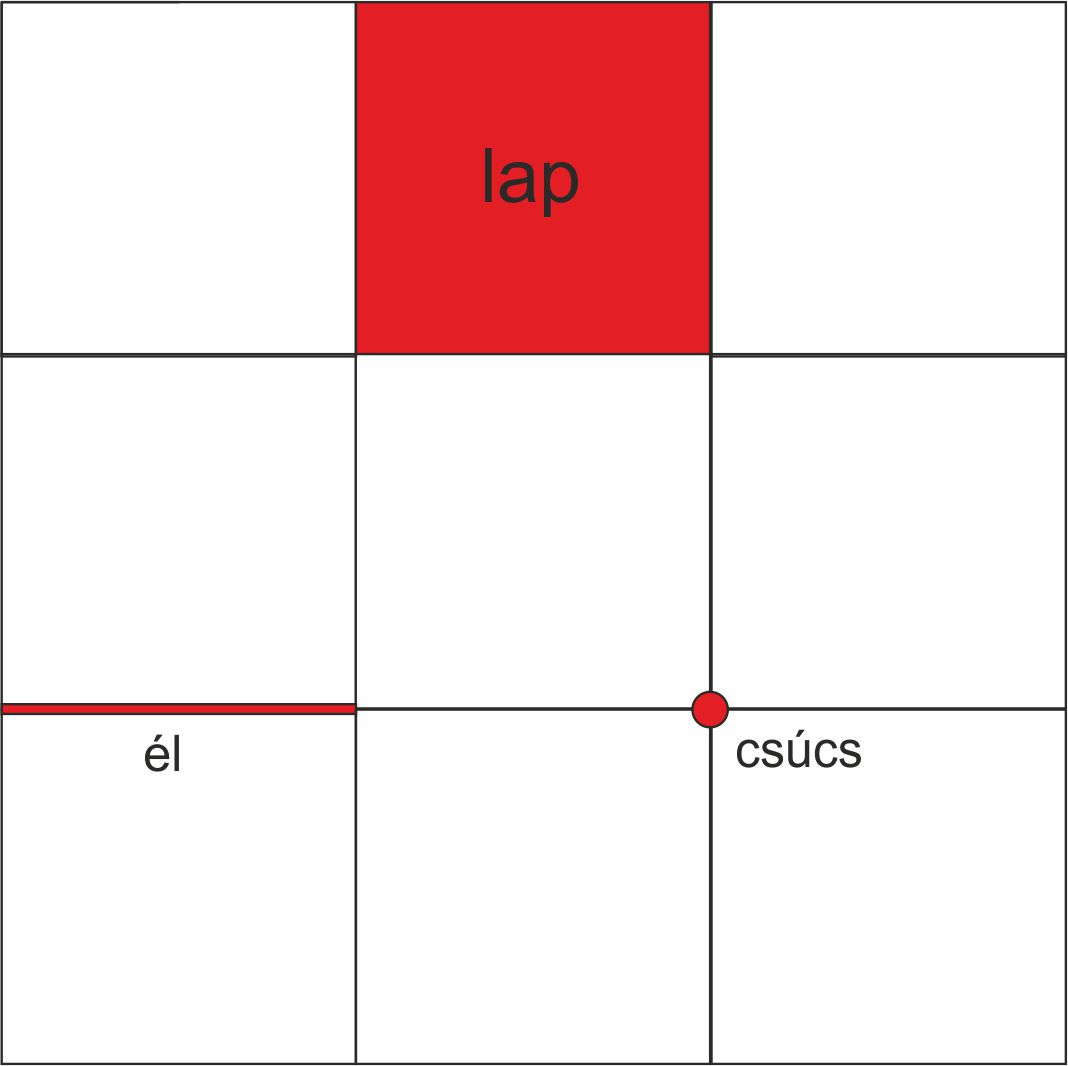
\includegraphics[scale=0.35]{kepek/PartsOfGrid.jpg}
\caption{A rács részei}
\label{fig:PartsOfGrid}
\end{figure}

A játékok nagy többségében közös az, hogy a rácsoknak csak az egyik részére koncentrálnak. A nyugati játékoknál mint a sakk vagy a dáma a rácsnak a lap részén van a fókusz ellentétben a keleti játékokkal mint a Go vagy a Csillaghalma (\textit{Chinese Checkers}), ahol a csúcsokon van (\ref{fig:PartsOfGrid2}. ábra).

Lapok, élek és csúcsok feltűnnek a különböző poligonokból álló térképek esetén is. Egy olyan algoritmus ami a lapok, élek vagy csúcsok alapján működik, de nincs szükség koordinátákra, az működni fog ilyen térképek esetén is.

\begin{figure}[h!]
\centering
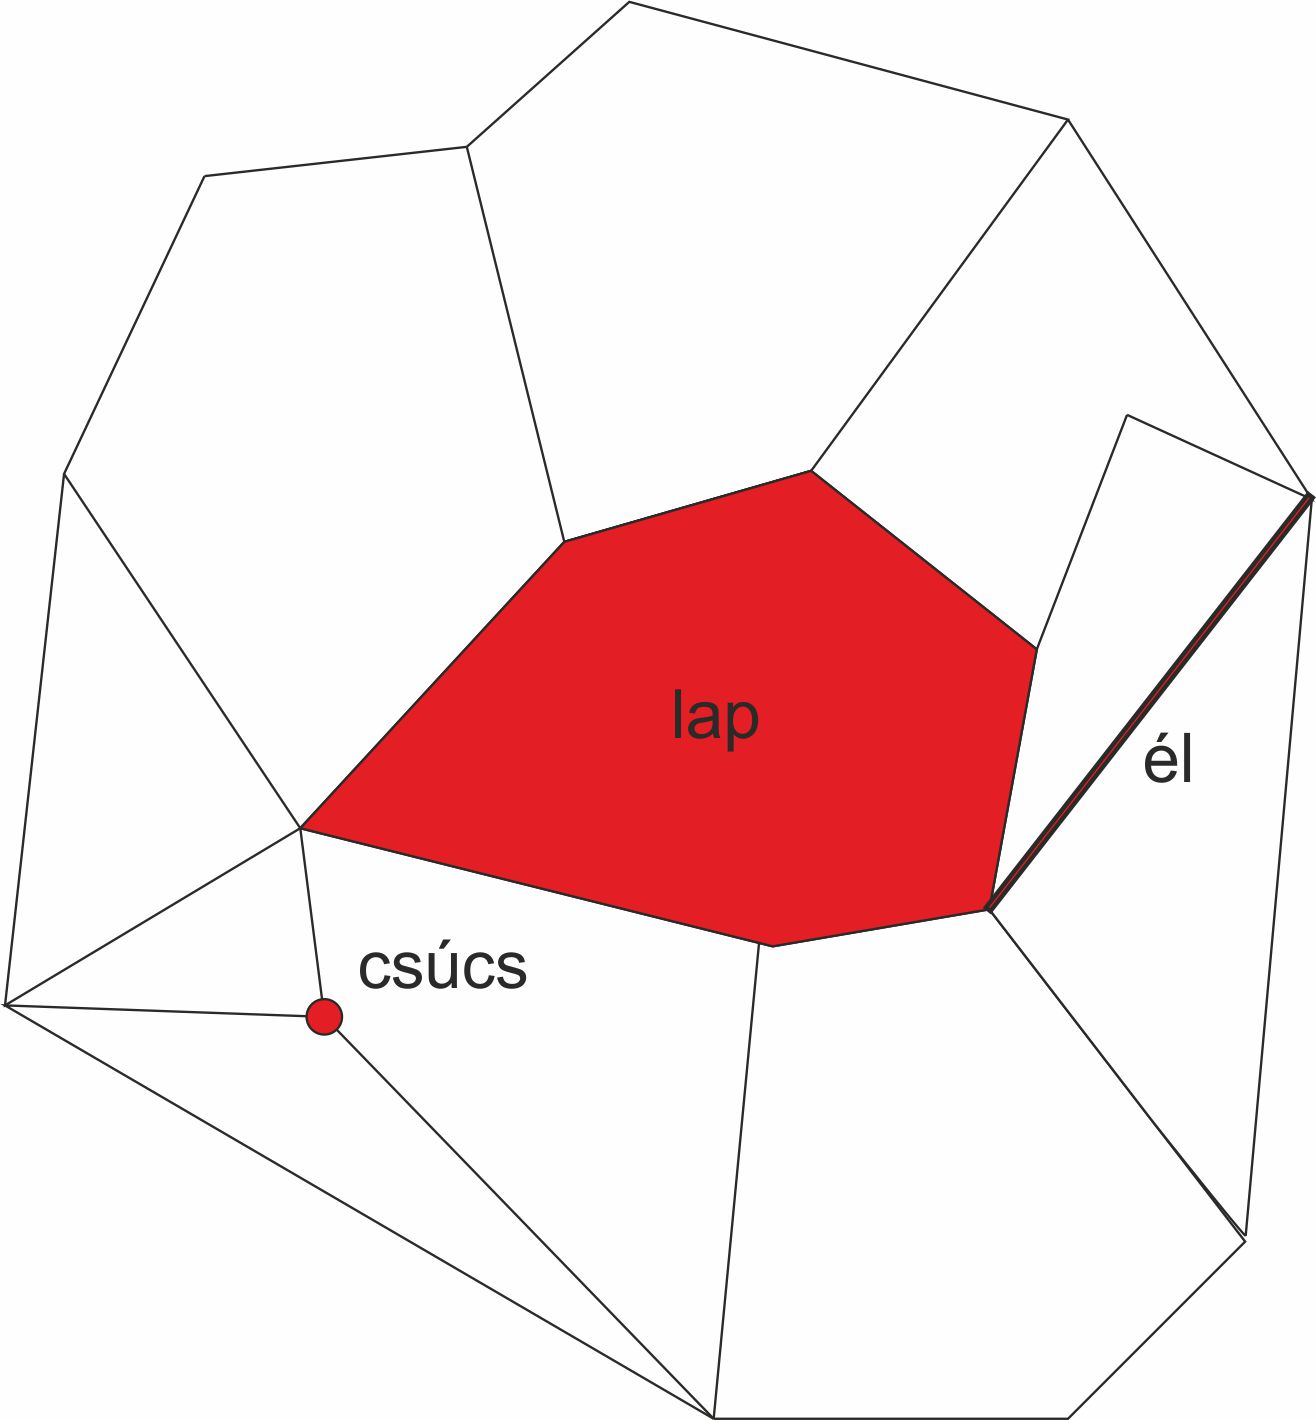
\includegraphics[scale=0.4]{kepek/PartsOfGrid2.jpg}
\caption{Különböző poligonokból álló térképen a rács részei}
\label{fig:PartsOfGrid2}
\end{figure}

A gráf struktúra megengedi számunkra, hogy gráf algoritmusokat (például legrövidebb utak számítását) használjunk a térképen. A rácsok és a poligonális térképek átalakíthatóak gráf struktúrákra azáltal, hogy minden lapból csomópontot és minden lapok között lévő élből pedig a csomópontokat összekötő éleket készítünk.

\section{Rácsok ábrázolása}

\subsection{Négyzetrácsok}

A négyzetháló esetén van a legkönnyebb dolgunk ismételten. A négyzeteket ebben az esetben úgy tudjuk egymás mellé helyezni, hogy a szomszédos négyzetek középpontjai közötti távolság megegyezik az oldal hosszal. 

Abban az esetben sincs sokkal nehezebb dolgunk, ha úgy döntünk, hogy az eltolt négyzetrácsos megoldást választjuk, ebben az esetben minden páros/páratlan sort/oszlopot kell eltolnunk az oldalak hosszának felével.

\subsection{Hexagonális rácsok}

A hexagonok alapvetően kétféleképpen állhatnak. Az egyik lehetőség, hogy az egyik csúcs van felül, a másik lehetőség, hogy az egyik oldal van felül. A klasszikus, két dimenziós játékok esetén külön figyelmet kell fordítani a rács irányultságára. A következő lépésként vizsgáljuk meg, hogy hogyan tudjuk egymás mellé elhelyezni a hexagonokat \cite{redblobgamesHexagonalGrids}.
\begin{itemize}
    \item A \textit{felül hegyes} elrendezés esetén vízszintesen a hexagon szélességével, függőlegesen pedig a hexagon magasságának a $\frac{3}{4}$ -vel kell eltolni a következő hexagont. Ezen kívül minden páros/páratlan sort vízszintesen a szélesség felével kell még eltolni (\ref{fig:PointyTop}. ábra).
    
\begin{figure}[h!]
\centering
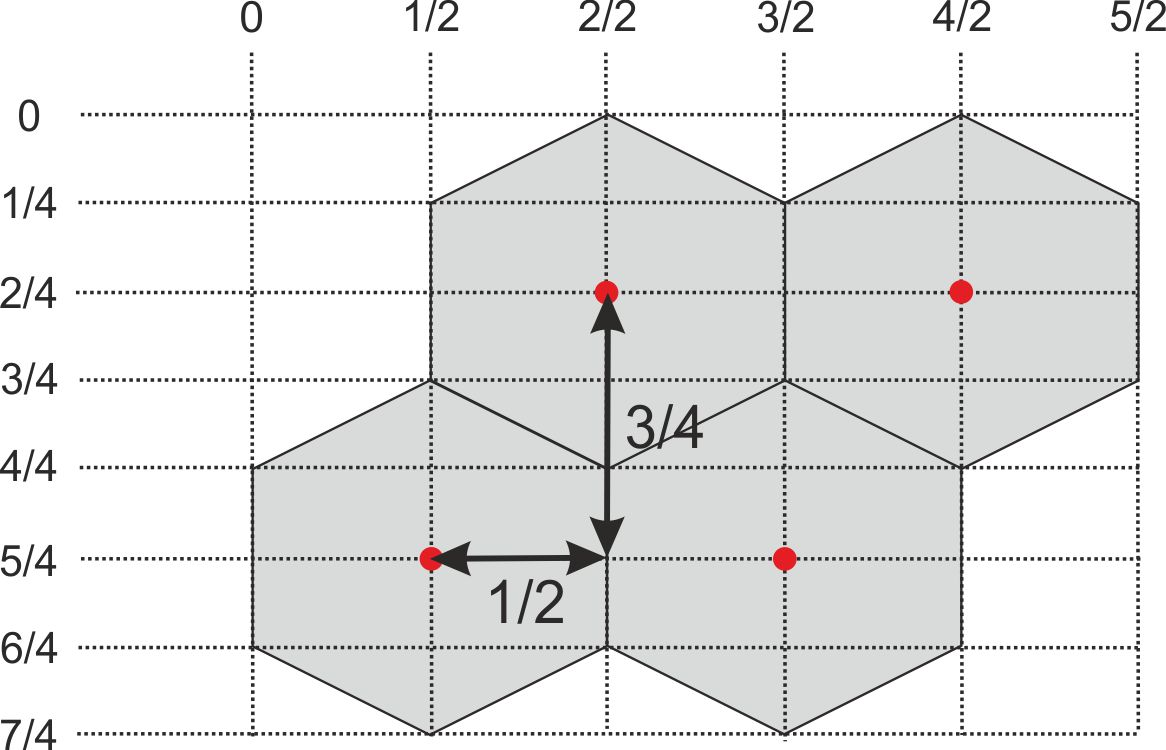
\includegraphics[scale=1.0]{kepek/PointyTop.jpg}
\caption{\textit{Felül hegyes} elrendezés esetén az eltolások}
\label{fig:PointyTop}
\end{figure}

    \item A \textit{felül lapos} elrendezés esetén vízszintesen az egymás melletti hexagonok közötti távolság a hexagon szélességének $\frac{3}{4}$ része. Függőlegesen minden páros/páratlan oszlopot a magasság felével kell eltolni (\ref{fig:FlatTop}. ábra).
\end{itemize}

\begin{figure}[h!]
\centering
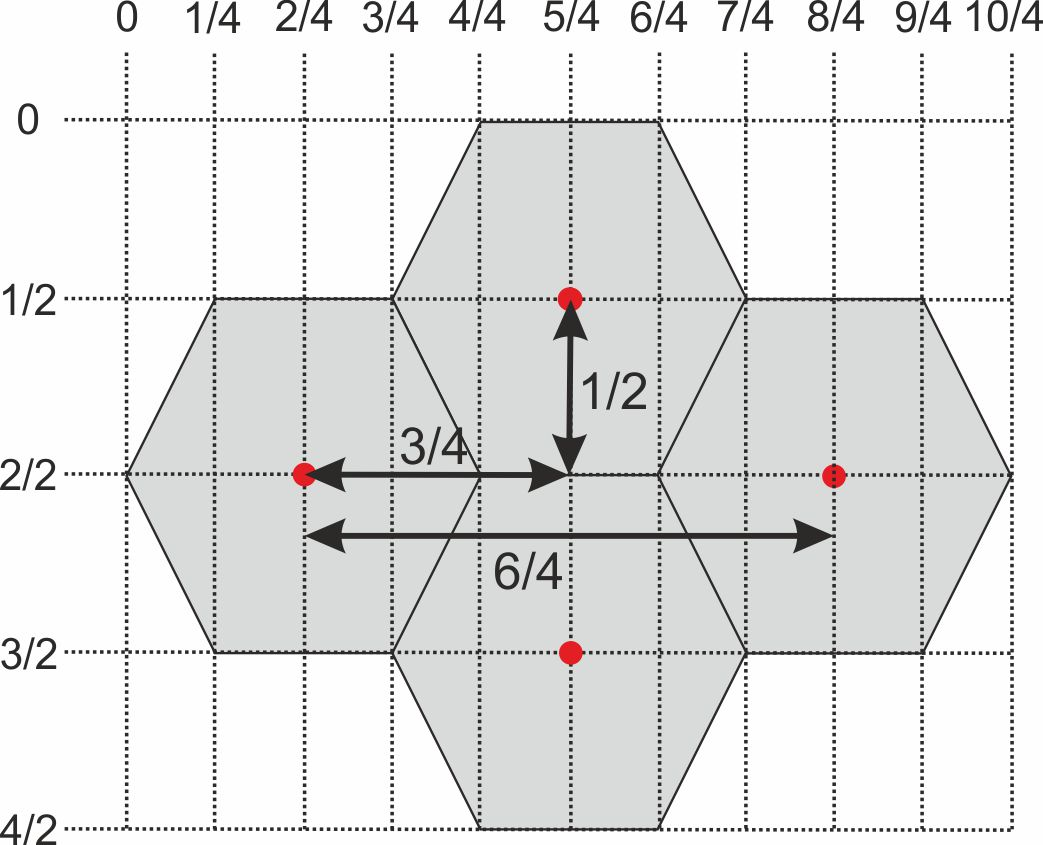
\includegraphics[scale=1.0]{kepek/FlatTop.jpg}
\caption{\textit{Felül lapos} elrendezés esetén az eltolások}
\label{fig:FlatTop}
\end{figure}

% TODO: Ide még kellene valamilyen zárszó féle, mert elég hirtelen végeszakadt a fejezetnek!

